
\section{Approach}
\label{sec:method}

Figure~\ref{fig:overview} represents the overview of 
tractability process, which includes four major steps
as follow:
\begin{enumerate}
	\item the grammatical tagging of the textual information of
	source and test files.
	\item the conversion of tagged files to 
	extensible markup language (XML).
	\item the generation of tractability links among 
	src-to-src, src-to-tst, and tst-to-tst files.
	\item search the source files to identify the
	 corresponding modules and test to portion a code changes.
	\item results filtering and evaluation. 
\end{enumerate}


\begin{figure}[!ht]
	\centering
	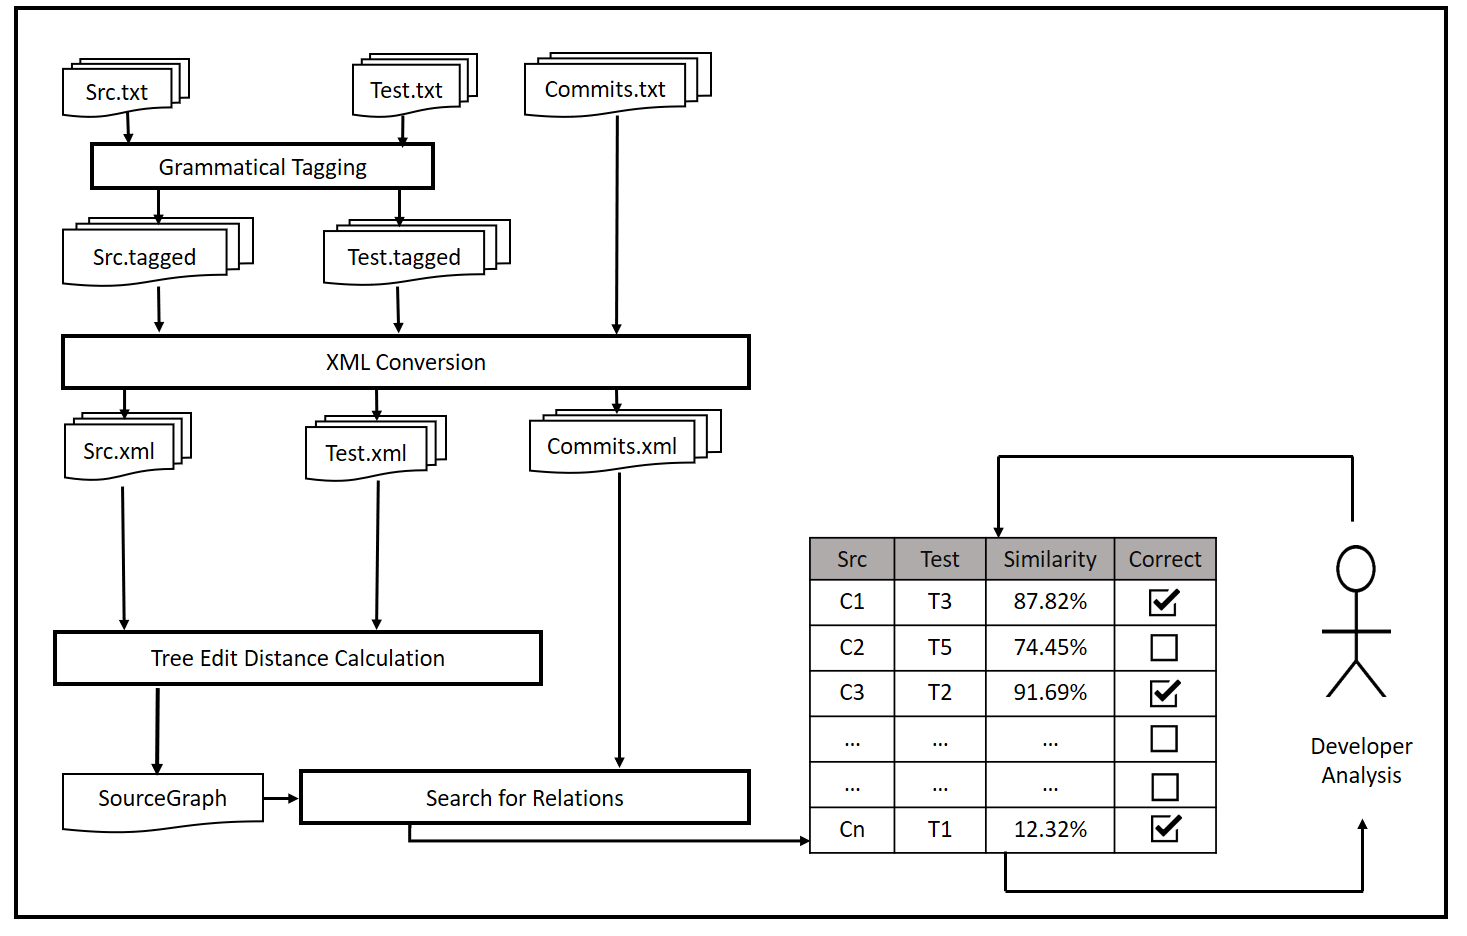
\includegraphics[width=0.95\linewidth]{./overview3.png}
	\vspace*{-10pt}
	\caption{The Traceability Process}
	\label{fig:overview}
	%	\vspace*{-10pt}
\end{figure}

Below we explain each step in details.


\subsection{Grammatical Tagging}
The source and test files are usually 
written in structured forms of their programming 
languages.  For instance, a class initially 
consist of libraries, variables, parameter, methods, etc. 
However, these parts of source files might vary 
depending on the grammatical rules of the programming languages.

Because our initial concern is to build a language independent 
system, we need to find a way to interpret each specific term 
into a common tag that will transfer the same meaning for each language. 
Therefor, our tagging process contains following steps:
The first step, the parser read the document files and identifies 
the file type, which can be a class, a library, a test class, etc.
In the next step, initial tags are assigned to the words based on
a lexicon and tagging rules. Then, the initial tags may be revised to 
take into account the context of words based on rules.  
For example, if a $<name>$ tag is followed by parenthesis in a
source file, this tag name will be updated to a $<function>$ tag
(see fig~\ref{fig:xml}).


\begin{figure*}[!ht]
	\centering
	\includegraphics[width=0.90\linewidth]{./xml2.png}
	\vspace*{-3pt}
	\caption{XML representation of the source code and test 
		cases of figure~\ref{fig:class} with their traceability relations}
	\label{fig:xml}
	%	\vspace*{-10pt}
\end{figure*}


\subsection{XML Conversion}

Once we built the tagged source code documents, we then 
transform each file into an equivalent XML document. 
Each XML document is structured according to the file type
and contains elements that are used to illustrate 
the structure of the source files 
(e.g. elements that identify the abstract syntax tree (AST),
in a source file that specify the 
parameters, methods, libraries, etc). 
The structure of source files and code commit would be similar 
because code commits are the modified versions of source files.
Test files, however, include additional tags, which are related to 
the unit testing such as asserts, target class/method, etc. 


Figure~\ref{fig:xml}, shows the XML representation 
of the source and test methods of Figure~\ref{fig:class}.
This representation reflects the structure of the original code structure.
For instance, the description of the
imported libraries of the class is enclosed 
in the XML element $<import> </import>$. 
It represent the tags that have been assigned 
to individual key terms for each programming language 
(e.g. static, public, return, etc).
Test files are converted to XML format in a similar way to the source files.


\subsection{Tractability Link Generation}
The next step is generating traceability links among the XML files. 
These set of relations are generated based on the analysis of 
the content of XML files, which are defined based on specific 
rules that we defined. 
To build these relations, we have specified the relations
in three different categories as follows:

\begin{enumerate}
	
	\item src-to-src dependency: 
	These set of dependencies are designed to determine the
	relations among source files, which specify the way of matching syntactically 
	related terms in the textual parts of a source file  with semantically 
	related elements of the other source files.
	
	Due to the different of grammatical and tagging structure of 
	each programming language, matching at this stage may also
	be informed by synonym lexicons. 
	For example, $\#include <x>$ in c language is equivalent to 
	$import \: x$  in Java. 
	The synonym lexicon file will interpret all 
	related terms to a single unique tag
	(e.g. $<import> </import>$ represent library import 
	regardless of their initial programming language). 
	
	
%	links source files to each other based on term similarities 
%	such as name, function name, parameter names, etc..

	\item tst-to-src dependency: 
	Relational links between test and source files are designed similar
	to the tst-to-tst link. However, the linkage
	are between source and test files. 
	In order to identify whether a test case can be 
	related to a source file we use the same notion, which 
	is whether the same string parameter has appeared in
	both files. 
	The underlying hypothesis is that
	we assume that specific term could be a function or
	parameter name and if it appears in both test 
	and source file it means that this test 
	exercise that portion of the source code. 
	
	\item tst-to-tst dependency: 	
	The other type of traceability relations are among test cases, 
	which can be the relations between separate test methods of 
	a single or different test classes.  
	Similarly to other dependencies, these dependency 
	links are specified in XML ($test-links.xml$). 
	The condition that may be used to specify the
	tst-to-tst is whether two string parameters are equal in 
	two different test cases. Therefore, we can generate a relational link
	between these two test cases.
	Figure~\ref{fig:xml} shows an example of how test cases can 
	be related to each other. 
	
	
%	links the test files to source files based on term similarity. 

	
%	links the test files to each other based on term similarity using edit distance. 
	
	
\end{enumerate}

All above mentioned types of dependencies 
are generated using Tree Edit Distance 
(details are explained in ~\ref{sec:tree}). 
%Below, we explain each set of relations in detail. 


%
%\subsubsection{src-to-src rules}
%These set of dependencies are designed to determine the
%relations among source files, which specify the way of matching syntactically 
%related terms in the textual parts of a source file  with semantically 
%related elements of the other source files.
%
%
%%To design these rules we defined a set of conditions and 
%%SANI checks whether these conditions are satisfied by the 
%%input files, then it will generate traceability links between 
%%these files.
%
%Due to the different of grammatical and tagging structure of 
%each programming language, matching at this stage may also
%be informed by synonym lexicons. 
%For example, $\#include <x>$ in c language is equivalent to 
%$import \: x$  in Java. 
%The synonym lexicon file will interpret all 
%related terms to a single unique tag
%(e.g. $<import> </import>$ represent library import 
%regardless of their initial programming language). 
%
%
%%The traceability links which are generated, represented in XML 
%%format and stored in the XML documents $src-to-src-relations.xml$. 
%%The set of conditions $C$ that may be used to specify the
%%src-to-src rules includes:
%%
%%
%%\begin{smallitem}
%%	\item {ASSOCIATION-OF (param1 , param2):}
%%	This condition is true if the param1 is a function, and 
%%	the param2 is a class, and param1 is 
%%	defined in or inherited by param2.
%%	
%%	\item {SUPERCLASS-OF (param1 , param2):}
%%	This condition is true if param1 is a class, and param2 is a 
%%	class, and param1 is a super class of param2.
%%	
%%	\item {ATTRIBUTE-OF (param1 , param2):}
%%	This condition is true if the param1 is an attribute, and param2 
%%	is a class, and param1 is defined in or inherited by param2.
%%\end{smallitem}
%
%
%\subsubsection{tst-to-tst links}
%
%The other type of traceability relations are among test cases, 
%which can be the relations between separate test methods of 
%a single or different test classes.  
%%The generation of traceability relations at this stage of the process is the 
%%result of the interpretation of a set of defiled rules for test files. 
%%These rules do not require an analysis of the text in the involved documents. 
%%They check for only the existence of particular types of traceability relations 
%%between these documents and generate additional traceability relations between 
%%the documents subject to the existence of such relations.
%Similarly to other dependencies, these dependency links are specified in XML ($test-links.xml$). 
%The condition that may be used to specify the
%tst-to-tst is whether two string parameters are equal in 
%two different test cases. Therefore, we can generate a relational link
%between these two test cases.
%Figure~\ref{fig:xml} shows an example of how test cases can 
%be related to each other. 
%
%
%%\begin{smallitem}
%%	\item{Overlap (param1 , param2):}
%%	 This condition becomes true if param1 in a test class/method and
%%	 param2 in another test class/method are equal.
%%	
%%	\item {Requires-Feature-In (param1 , param2):}
%%	This condition becomes true if the param1 is a test method, and 
%%	the param2 is a test class, and param1 requires a attribute in param2.
%%	
%%	\item {CONTAINS (str1 , str2):}
%%	This condition becomes true if str2 is a substring of str1.
%%	
%%	\item {EQUAL-TO (str1 , str2):}
%%	This condition becomes true if str2 is a equal to str1.
%%\end{smallitem}
%
%
%
%\subsubsection{tst-to-src rules}
%
%Relational links between test and source files are designed similar
%to the tst-to-tst link. However, the linkage
%are between source and test files. 
%In order to identify whether a test case can be 
%related to a source file we use the same notion, which 
%is whether the same string parameter has appeared in
%both files. 
%The underlying hypothesis is that
%we assume that specific term could be a function or
%parameter name and if it appears in both test 
%and source file it means that this test 
%exercise that portion of the source code. 
%
%%The set of the conditions that may be used to specify the
%%tst-to-src rules includes:
%%
%%\begin{smallitem}
%%	\item{Overlap (param1 , param2):}
%%	This condition becomes true if param1 in a test method and
%%	param2 in source file are equal.
%%	
%%	\item {Requires-Feature-In (param1 , param2):}
%%	This condition becomes true if the param1 is a test method, and 
%%	the param2 is a source file, and param1 requires a attribute in param2.
%%	
%%	\item {CONTAINS (str1 , str2 ):}
%%	This predicate becomes true if str2 of a test method is 
%%	a sub-string of str1 of a source file.
%%	
%%	\item {EQUAL-TO (str1 , str2 ):}
%%	This predicate becomes true if str2 of a test method is 
%%	equal to str1 of a source file.
%%
%%\end{smallitem}



%\subsubsection{Query construction}
%\label{sec:query}
%




\subsubsection{Source Graph Generation and Search Algorithm}
\label{sec:tree}


First we need to generate the relational links among source
to test cases, we then build a graph in which the nodes
are source files and test cases and the edges represent 
the relation among the nodes.
Figure~\ref{fig:graph} shows an example of generated 
source graph. 
Because the initial goal of our approach is to 
automate the regression test case prioritization, we need to 
search among the source graph to determine the
portion of the source code that correspond to the
code changes.  
To do that, we use the code changes 
between two program versions that we have converted them to 
XML files (see Fig~\ref{fig:class} and~\ref{fig:xml})
as a input for the search in the source graph. 

\begin{figure*}[!ht]
	\centering
	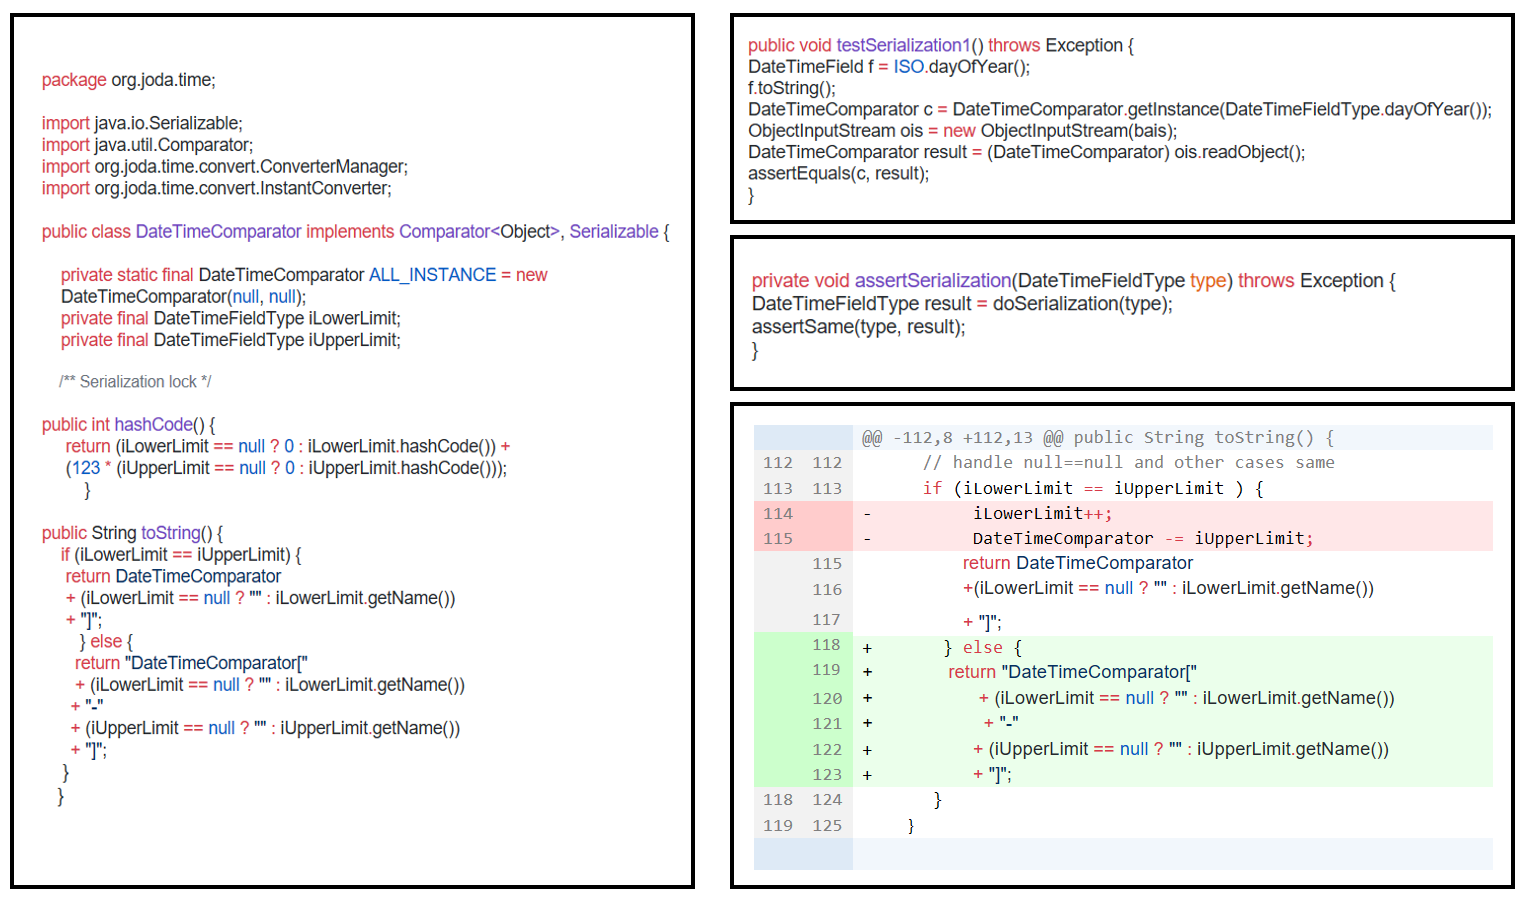
\includegraphics[width=0.90\linewidth]{./allcodes2.png}
	\vspace*{-3pt}
	\caption{An example of class, two test case, and a code commit. 
		testSerilization() is 
		from TestDateTimeComparator.java class, and assertSeilization() is from
		TestDateTimeFieldType.java class.}
	\label{fig:class}
\end{figure*}

The tree edit distance algorithm is a widely used technique 
by researcher to compare semi-structured data,
such as XML documents~\cite{xml, treeedit}. 
Therefore, we apply this algorithm to 
calculate the similarity between code commits and each source file.
This algorithm find the minimal cost 
sequence of edit operation that can transfer a labeled tree
to another one. 
More formally, for a given labeled tree T where each node 
is a symbol from a fixed finite alphabet $\sum$.
We call T an ordered tree if a left-to-right
order among siblings in T is given. The matching problems is
simple primitive operations applied to labeled trees. 
For an ordered tree T, these set of edit operations are:

\begin{smallitem}
	\item{rename:} Change the label of a vertex v in T.
	\item{delete:} Delete a non-root vertex v in T with parent v', 
	making the children of v become the children of v'.
	\item{insert:} Insert a vertex v as a child of v'
	in T making v the parent of a consecutive subsequence of the children of v'.
	
\end{smallitem}

For a given cost function defined for
each edit operation. An edit distance D 
between T1 and T2 is a sequence of edit
operations turning T1 into T2. 
The cost of D is the sum of the costs of the
operations in D. The tree edit distance problem is to 
calculate the edit distance and a corresponding edit script~\cite{treeedit}.
Once we identify the corresponding portion of the code, 
we then select all linked test cases that are directly or indirectly 
exercising that portion of the code change.
Below we explain test selection process in detail.

\begin{figure}[!ht]
	\centering
	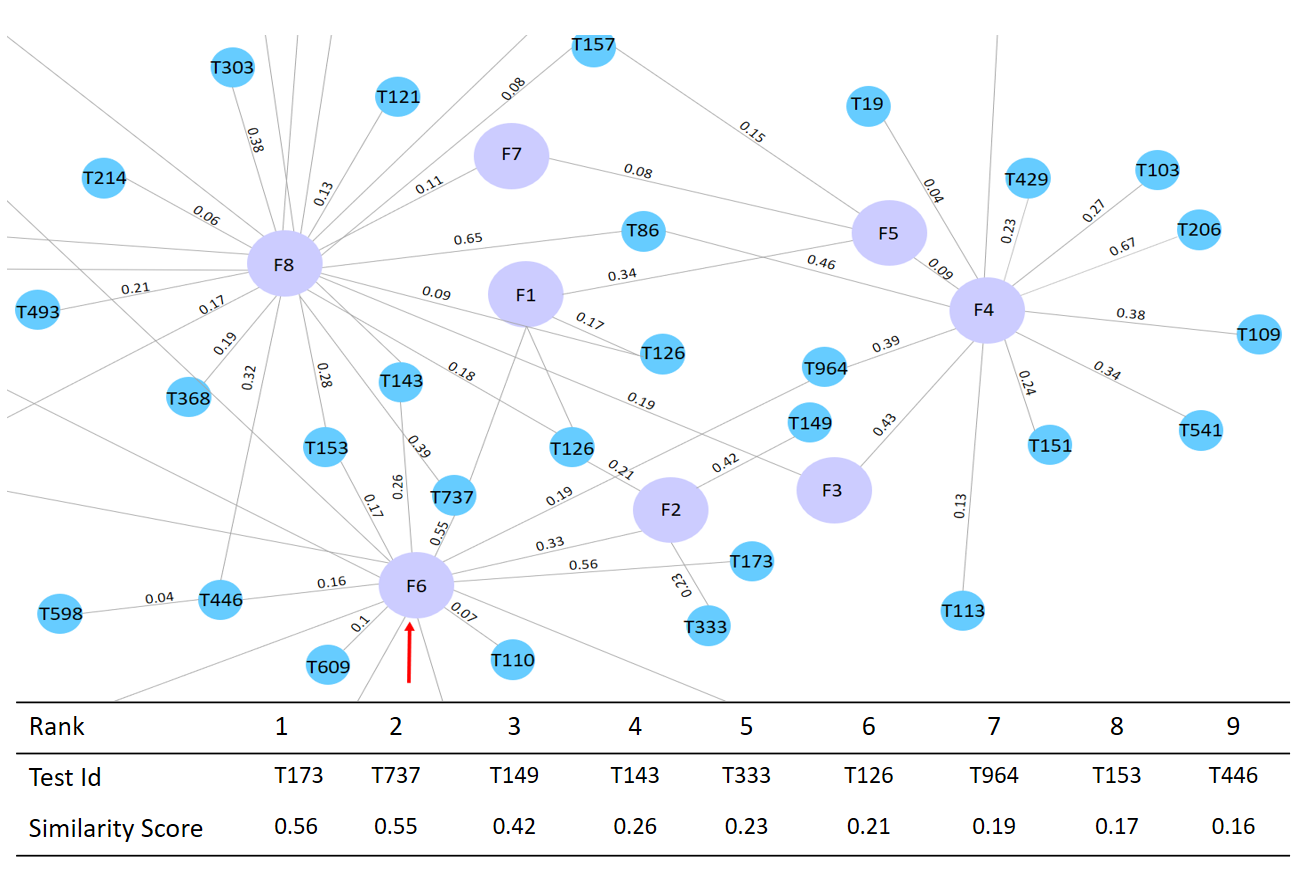
\includegraphics[width=0.90\linewidth]{./networklayout.png}
%	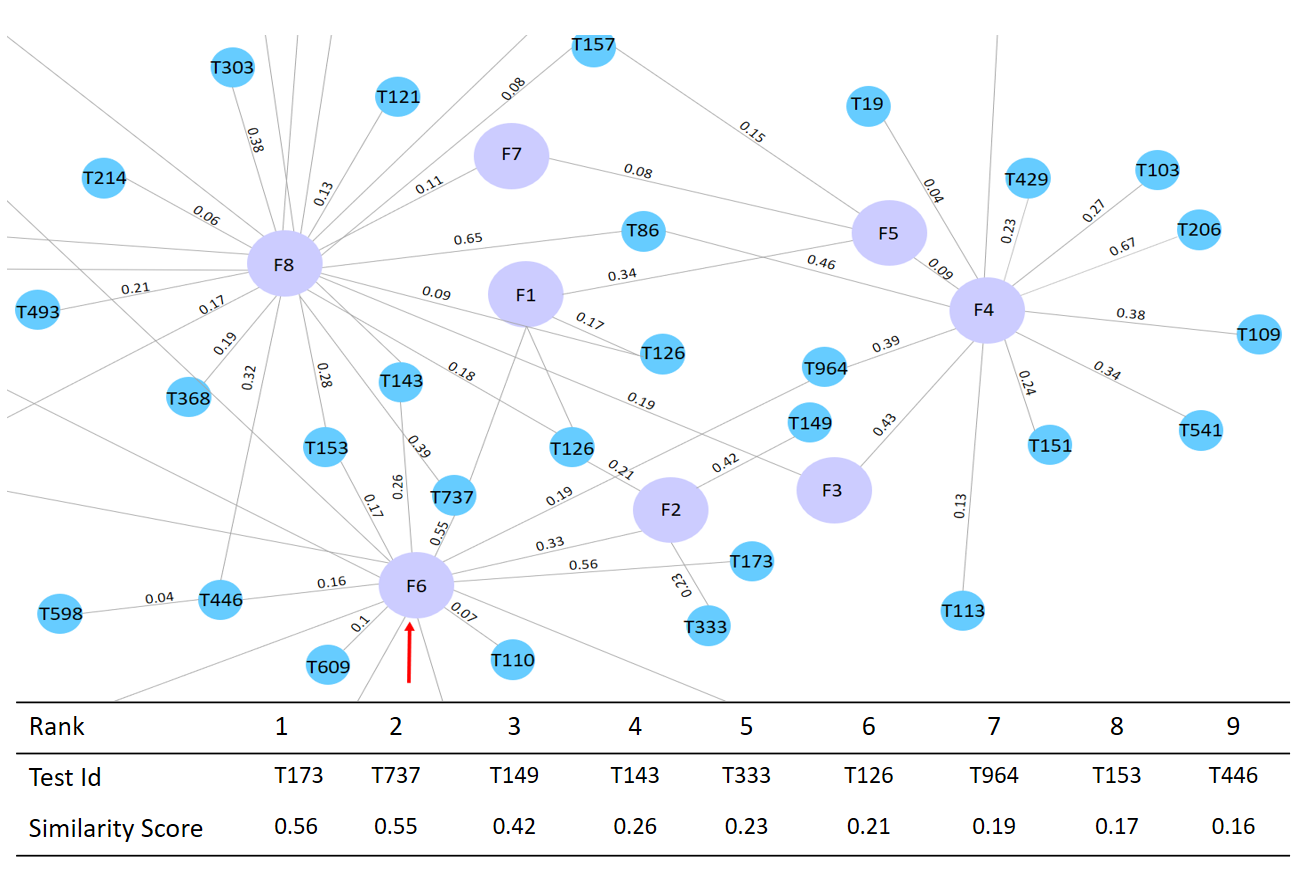
\includegraphics[width=70mm,scale=0.8]{./networklayout.png}
	\vspace*{-5pt}
	\caption{An Example of Source Graph Network Layout}
	\label{fig:graph}
	\vspace*{-10pt}
\end{figure}



Figure~\ref{fig:graph} represents an example 
of the generated source code graph. In this example, 
if function f6 has been modified (pointed with an array), 
therefor its change can impact function f2 too because 
f2 is dependent on f6. 
GTXCrawler starts with identifying all 
related test cases to the modified file and
all other files that are dependent on the modified 
file (in this case F2). It then returns a report of the
dependent test cases with their similarity scores. 
At this point developer reviews the test cases to evaluate 
a suitable similarity scores that can be a good indicator 
to the test files and filters out those that not related.
Generally, the higher similarity scores indicates that 
there is a higher correlation between files. 

Assume that developer set the minimum similarity score to 0.15,
which means that only test cases that meet this minimum 
score should be selected. 
GTXCrwaler then reorder the test cases in this way:
first it selects all dependent test cases to both F6 and F2 
that can satisfy the minimum similarity score, it then 
prioritizes the test cases based on their similarity scores.
The test cases that have higher similarity score will be 
selected earlier because we hypothesis that those test cases
have higher correlation to the modified files. 
Therefore,  the set of test cases to be selected first is T173, 
T737, T149, T143, T333, T126, T964, T153, AND T446.









%%%%%%%%%%%% %%%%%%%%%%%%%%% maybe later

%how to build the document in tree % data orgnization
%
%Since all value entities in XML data are considered
%variable-length character strings, all distinct name strings
%are collected in the name index, which is implemented as
%a B +-tree. Then, each distinct name string is uniquely
%identified by a name identifier (or nid) returned from the
%name index. The use of name index minimizes storage
%and computational overhead by eliminating replicated
%strings and string comparisons. For the same reason, all
%string values (i.e. attribute value and text value) are 
%collected in value table. Each XML document is also 
%assigned a unique document identifier (did), which is an
%index key to retrieve the document name. An element or
%attribute can be uniquely identified by its order and did
%in the entire system.
%
%The element index, attribute index and structure index
%are the three indexes to support the three essential 
%functionalities listed above, respectively. Both the element
%index and attribute index are implemented as a B +-tree
%using name identifiers (nid) as keys. Each entry in a leaf
%node points to a set of fixed-length records for elements
%(or attributes) having an identical name string, grouped
%by document they belong to. The element index allows
%us to quickly find all elements with the same name string,
%which is one of the most common operations to process
%regular path expression queries. Each element record
%includes an < order ; size > pair and other related 
%information of the element, and the element records are in a
%sorted order by the order values as shown in Figure 3.
%
%The attribute index has almost the same structure as
%the element index, except that the record in attribute 
%index has a value identifier vid, which is a key used 
%to obtain the attribute value from the value table.

